\begin{enunciado}{2}
    Show that for the learning model of positive rectangles (aligned horizontally or vertically), $m_{\hipotset}(4) = 2^4$ and $m_{\hipotset}(5) < 2^5$. Hence, give a bound for $m_{\hipotset}(N)$.
\end{enunciado}

Let’s try rectangles with horizontal and vertical edges. In order to show that the VC dimension is 4 (in this
case), we need to show two things:
1. There exist 4 points that can be shattered.
It’s clear that capturing just 1 point and all 4 points are both trivial. The figure below shows how we
can capture 2 points and 3 points.

\begin{figure}[h]
\centering
\begin{minipage}{0.46\textwidth}
\centering
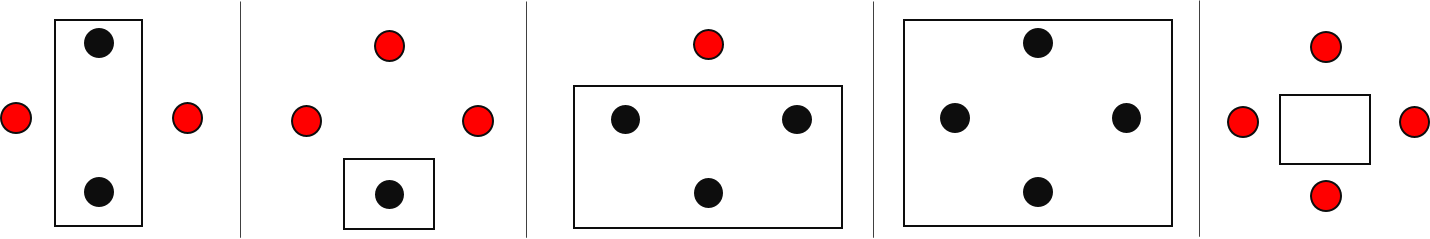
\includegraphics[width=\textwidth]{images/2-2-dvc4.png}
\caption{$\dvc = 2$}
\end{minipage}